\documentclass{standalone}
\usepackage{tikz}
\usetikzlibrary{patterns, positioning}

\begin{document}
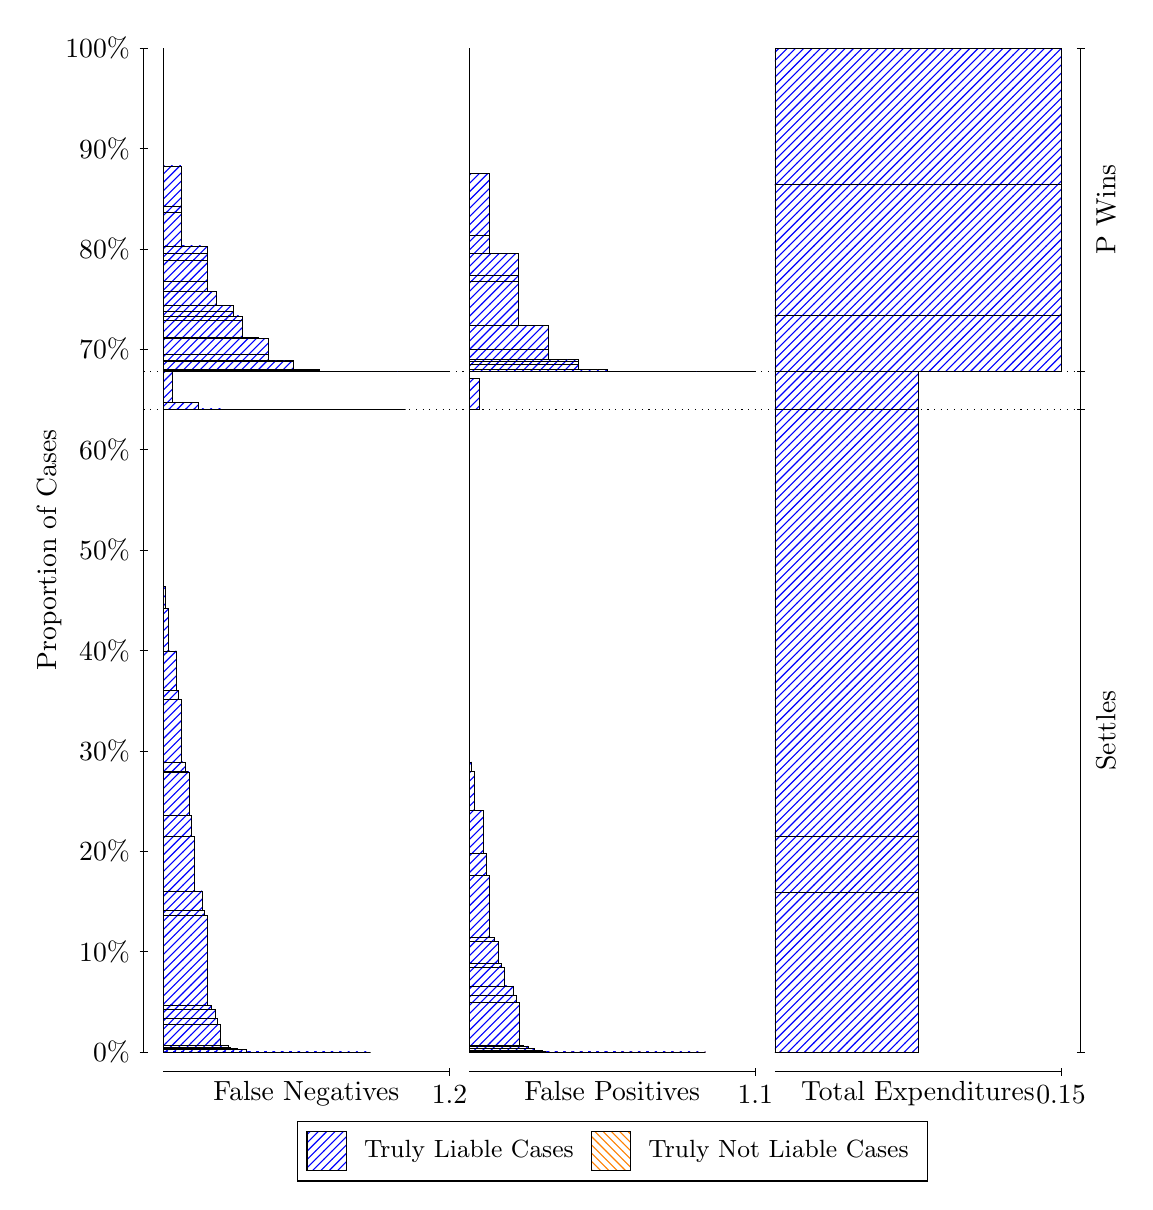
\begin{tikzpicture}
\draw[black, very thin] (1.5,1.75) -- (1.5,14.5);
\node[rotate=90, anchor=center] at (0.3, 8.125) {Proportion of Cases};
\draw[black, very thin] (1.45,1.75) -- (1.55,1.75);
\node[anchor=east] at (1.45, 1.75) {0\%};
\draw[black, very thin] (1.45,3.025) -- (1.55,3.025);
\node[anchor=east] at (1.45, 3.025) {10\%};
\draw[black, very thin] (1.45,4.3) -- (1.55,4.3);
\node[anchor=east] at (1.45, 4.3) {20\%};
\draw[black, very thin] (1.45,5.575) -- (1.55,5.575);
\node[anchor=east] at (1.45, 5.575) {30\%};
\draw[black, very thin] (1.45,6.85) -- (1.55,6.85);
\node[anchor=east] at (1.45, 6.85) {40\%};
\draw[black, very thin] (1.45,8.125) -- (1.55,8.125);
\node[anchor=east] at (1.45, 8.125) {50\%};
\draw[black, very thin] (1.45,9.4) -- (1.55,9.4);
\node[anchor=east] at (1.45, 9.4) {60\%};
\draw[black, very thin] (1.45,10.675) -- (1.55,10.675);
\node[anchor=east] at (1.45, 10.675) {70\%};
\draw[black, very thin] (1.45,11.95) -- (1.55,11.95);
\node[anchor=east] at (1.45, 11.95) {80\%};
\draw[black, very thin] (1.45,13.225) -- (1.55,13.225);
\node[anchor=east] at (1.45, 13.225) {90\%};
\draw[black, very thin] (1.45,14.5) -- (1.55,14.5);
\node[anchor=east] at (1.45, 14.5) {100\%};

\draw[black, very thin] (13.4,1.75) -- (13.4,14.5);
\draw[black, very thin] (13.35,1.75) -- (13.45,1.75);
\node[anchor=west] at (13.35, 1.75) {};
\draw[black, very thin] (13.35,9.9125) -- (13.45,9.9125);
\node[anchor=west] at (13.35, 9.9125) {};
\draw[black, very thin] (13.35,10.394) -- (13.45,10.394);
\node[anchor=west] at (13.35, 10.394) {};
\draw[black, very thin] (13.35,14.5) -- (13.45,14.5);
\node[anchor=west] at (13.35, 14.5) {};

\draw[black, very thin, pattern color=blue, pattern=north east lines] (1.75,1.75) rectangle (4.3823,1.75);
\draw[black, very thin, pattern color=blue, pattern=north east lines] (1.75,1.75) rectangle (4.0857,1.75);
\draw[black, very thin, pattern color=blue, pattern=north east lines] (1.75,1.75) rectangle (4.0528,1.75);
\draw[black, very thin, pattern color=blue, pattern=north east lines] (1.75,1.75) rectangle (3.7891,1.75);
\draw[black, very thin, pattern color=blue, pattern=north east lines] (1.75,1.75) rectangle (3.7562,1.75);
\draw[black, very thin, pattern color=blue, pattern=north east lines] (1.75,1.75) rectangle (3.7232,1.75);
\draw[black, very thin, pattern color=blue, pattern=north east lines] (1.75,1.75) rectangle (3.6408,1.75);
\draw[black, very thin, pattern color=blue, pattern=north east lines] (1.75,1.75) rectangle (3.4596,1.75);
\draw[black, very thin, pattern color=blue, pattern=north east lines] (1.75,1.75) rectangle (3.4266,1.75);
\draw[black, very thin, pattern color=blue, pattern=north east lines] (1.75,1.75) rectangle (3.3937,1.75);
\draw[black, very thin, pattern color=blue, pattern=north east lines] (1.75,1.75) rectangle (3.3442,1.75);
\draw[black, very thin, pattern color=blue, pattern=north east lines] (1.75,1.75) rectangle (3.3113,1.75);
\draw[black, very thin, pattern color=blue, pattern=north east lines] (1.75,1.75) rectangle (3.13,1.7505);
\draw[black, very thin, pattern color=blue, pattern=north east lines] (1.75,1.7505) rectangle (3.0971,1.7506);
\draw[black, very thin, pattern color=blue, pattern=north east lines] (1.75,1.7506) rectangle (3.0641,1.7507);
\draw[black, very thin, pattern color=blue, pattern=north east lines] (1.75,1.7507) rectangle (3.0476,1.7507);
\draw[black, very thin, pattern color=blue, pattern=north east lines] (1.75,1.7507) rectangle (3.0147,1.7508);
\draw[black, very thin, pattern color=blue, pattern=north east lines] (1.75,1.7508) rectangle (2.9817,1.7508);
\draw[black, very thin, pattern color=blue, pattern=north east lines] (1.75,1.7508) rectangle (2.8993,1.7519);
\draw[black, very thin, pattern color=blue, pattern=north east lines] (1.75,1.7519) rectangle (2.8005,1.7781);
\draw[black, very thin, pattern color=blue, pattern=north east lines] (1.75,1.7781) rectangle (2.7675,1.7835);
\draw[black, very thin, pattern color=blue, pattern=north east lines] (1.75,1.7835) rectangle (2.7345,1.7892);
\draw[black, very thin, pattern color=blue, pattern=north east lines] (1.75,1.7892) rectangle (2.7181,1.7894);
\draw[black, very thin, pattern color=blue, pattern=north east lines] (1.75,1.7894) rectangle (2.6851,1.7944);
\draw[black, very thin, pattern color=blue, pattern=north east lines] (1.75,1.7944) rectangle (2.6522,1.7946);
\draw[black, very thin, pattern color=blue, pattern=north east lines] (1.75,1.7946) rectangle (2.6027,1.8049);
\draw[black, very thin, pattern color=blue, pattern=north east lines] (1.75,1.8049) rectangle (2.5698,1.8344);
\draw[black, very thin, pattern color=blue, pattern=north east lines] (1.75,1.8344) rectangle (2.4709,2.0985);
\draw[black, very thin, pattern color=blue, pattern=north east lines] (1.75,2.0985) rectangle (2.4379,2.1723);
\draw[black, very thin, pattern color=blue, pattern=north east lines] (1.75,2.1723) rectangle (2.405,2.2912);
\draw[black, very thin, pattern color=blue, pattern=north east lines] (1.75,2.2912) rectangle (2.3885,2.2936);
\draw[black, very thin, pattern color=blue, pattern=north east lines] (1.75,2.2936) rectangle (2.3556,2.3467);
\draw[black, very thin, pattern color=blue, pattern=north east lines] (1.75,2.3467) rectangle (2.3226,2.3491);
\draw[black, very thin, pattern color=blue, pattern=north east lines] (1.75,2.3491) rectangle (2.3061,3.4906);
\draw[black, very thin, pattern color=blue, pattern=north east lines] (1.75,3.4906) rectangle (2.2732,3.5515);
\draw[black, very thin, pattern color=blue, pattern=north east lines] (1.75,3.5515) rectangle (2.2402,3.7953);
\draw[black, very thin, pattern color=blue, pattern=north east lines] (1.75,3.7953) rectangle (2.1413,4.4853);
\draw[black, very thin, pattern color=blue, pattern=north east lines] (1.75,4.4853) rectangle (2.1084,4.7548);
\draw[black, very thin, pattern color=blue, pattern=north east lines] (1.75,4.7548) rectangle (2.0754,5.3074);
\draw[black, very thin, pattern color=blue, pattern=north east lines] (1.75,5.3074) rectangle (2.059,5.3131);
\draw[black, very thin, pattern color=blue, pattern=north east lines] (1.75,5.3131) rectangle (2.026,5.4296);
\draw[black, very thin, pattern color=blue, pattern=north east lines] (1.75,5.4296) rectangle (1.993,5.4353);
\draw[black, very thin, pattern color=blue, pattern=north east lines] (1.75,5.4353) rectangle (1.9766,6.2277);
\draw[black, very thin, pattern color=blue, pattern=north east lines] (1.75,6.2277) rectangle (1.9436,6.3457);
\draw[black, very thin, pattern color=blue, pattern=north east lines] (1.75,6.3457) rectangle (1.9107,6.8434);
\draw[black, very thin, pattern color=blue, pattern=north east lines] (1.75,6.8434) rectangle (1.8118,7.3894);
\draw[black, very thin, pattern color=blue, pattern=north east lines] (1.75,7.3894) rectangle (1.7788,7.6622);
\draw[black, very thin, pattern color=orange, pattern=north west lines] (1.75,7.6622) rectangle (1.75,7.6622);
\draw[black, very thin, pattern color=blue, pattern=north east lines] (1.75,7.6622) rectangle (1.75,9.9125);
\draw[black, very thin, pattern color=blue, pattern=north east lines] (1.75,9.9125) rectangle (4.8272,9.9125);
\draw[black, very thin, pattern color=blue, pattern=north east lines] (1.75,9.9125) rectangle (4.4977,9.9125);
\draw[black, very thin, pattern color=blue, pattern=north east lines] (1.75,9.9125) rectangle (4.1681,9.9125);
\draw[black, very thin, pattern color=blue, pattern=north east lines] (1.75,9.9125) rectangle (3.8385,9.9125);
\draw[black, very thin, pattern color=blue, pattern=north east lines] (1.75,9.9125) rectangle (3.509,9.9125);
\draw[black, very thin, pattern color=blue, pattern=north east lines] (1.75,9.9125) rectangle (3.1794,9.9125);
\draw[black, very thin, pattern color=blue, pattern=north east lines] (1.75,9.9125) rectangle (2.8499,9.9126);
\draw[black, very thin, pattern color=blue, pattern=north east lines] (1.75,9.9126) rectangle (2.5203,9.9173);
\draw[black, very thin, pattern color=blue, pattern=north east lines] (1.75,9.9173) rectangle (2.1908,10.003);
\draw[black, very thin, pattern color=blue, pattern=north east lines] (1.75,10.003) rectangle (1.8612,10.394);
\draw[black, very thin, pattern color=orange, pattern=north west lines] (1.75,10.394) rectangle (1.75,10.394);
\draw[black, very thin, pattern color=blue, pattern=north east lines] (1.75,10.394) rectangle (5.3833,10.394);
\draw[black, very thin, pattern color=blue, pattern=north east lines] (1.75,10.394) rectangle (5.0538,10.394);
\draw[black, very thin, pattern color=blue, pattern=north east lines] (1.75,10.394) rectangle (4.7242,10.394);
\draw[black, very thin, pattern color=blue, pattern=north east lines] (1.75,10.394) rectangle (4.6089,10.394);
\draw[black, very thin, pattern color=blue, pattern=north east lines] (1.75,10.394) rectangle (4.3947,10.394);
\draw[black, very thin, pattern color=blue, pattern=north east lines] (1.75,10.394) rectangle (4.2793,10.394);
\draw[black, very thin, pattern color=blue, pattern=north east lines] (1.75,10.394) rectangle (4.2793,10.394);
\draw[black, very thin, pattern color=blue, pattern=north east lines] (1.75,10.394) rectangle (4.0651,10.396);
\draw[black, very thin, pattern color=blue, pattern=north east lines] (1.75,10.396) rectangle (4.0651,10.397);
\draw[black, very thin, pattern color=blue, pattern=north east lines] (1.75,10.397) rectangle (3.9498,10.397);
\draw[black, very thin, pattern color=blue, pattern=north east lines] (1.75,10.397) rectangle (3.7356,10.408);
\draw[black, very thin, pattern color=blue, pattern=north east lines] (1.75,10.408) rectangle (3.7356,10.423);
\draw[black, very thin, pattern color=blue, pattern=north east lines] (1.75,10.423) rectangle (3.6202,10.423);
\draw[black, very thin, pattern color=blue, pattern=north east lines] (1.75,10.423) rectangle (3.406,10.521);
\draw[black, very thin, pattern color=blue, pattern=north east lines] (1.75,10.521) rectangle (3.406,10.538);
\draw[black, very thin, pattern color=blue, pattern=north east lines] (1.75,10.538) rectangle (3.2907,10.538);
\draw[black, very thin, pattern color=blue, pattern=north east lines] (1.75,10.538) rectangle (3.2907,10.538);
\draw[black, very thin, pattern color=blue, pattern=north east lines] (1.75,10.538) rectangle (3.0765,10.608);
\draw[black, very thin, pattern color=blue, pattern=north east lines] (1.75,10.608) rectangle (3.0765,10.812);
\draw[black, very thin, pattern color=blue, pattern=north east lines] (1.75,10.812) rectangle (2.9611,10.816);
\draw[black, very thin, pattern color=blue, pattern=north east lines] (1.75,10.816) rectangle (2.9611,10.823);
\draw[black, very thin, pattern color=blue, pattern=north east lines] (1.75,10.823) rectangle (2.9611,10.824);
\draw[black, very thin, pattern color=blue, pattern=north east lines] (1.75,10.824) rectangle (2.7469,10.829);
\draw[black, very thin, pattern color=blue, pattern=north east lines] (1.75,10.829) rectangle (2.7469,11.046);
\draw[black, very thin, pattern color=blue, pattern=north east lines] (1.75,11.046) rectangle (2.7469,11.098);
\draw[black, very thin, pattern color=blue, pattern=north east lines] (1.75,11.098) rectangle (2.6316,11.099);
\draw[black, very thin, pattern color=blue, pattern=north east lines] (1.75,11.099) rectangle (2.6316,11.16);
\draw[black, very thin, pattern color=blue, pattern=north east lines] (1.75,11.16) rectangle (2.6316,11.233);
\draw[black, very thin, pattern color=blue, pattern=north east lines] (1.75,11.233) rectangle (2.4173,11.407);
\draw[black, very thin, pattern color=blue, pattern=north east lines] (1.75,11.407) rectangle (2.302,11.536);
\draw[black, very thin, pattern color=blue, pattern=north east lines] (1.75,11.536) rectangle (2.302,11.81);
\draw[black, very thin, pattern color=blue, pattern=north east lines] (1.75,11.81) rectangle (2.302,11.888);
\draw[black, very thin, pattern color=blue, pattern=north east lines] (1.75,11.888) rectangle (2.302,11.986);
\draw[black, very thin, pattern color=blue, pattern=north east lines] (1.75,11.986) rectangle (2.0878,11.988);
\draw[black, very thin, pattern color=blue, pattern=north east lines] (1.75,11.988) rectangle (2.0878,11.988);
\draw[black, very thin, pattern color=blue, pattern=north east lines] (1.75,11.988) rectangle (1.9724,12.419);
\draw[black, very thin, pattern color=blue, pattern=north east lines] (1.75,12.419) rectangle (1.9724,12.495);
\draw[black, very thin, pattern color=blue, pattern=north east lines] (1.75,12.495) rectangle (1.9724,13.004);
\draw[black, very thin, pattern color=blue, pattern=north east lines] (1.75,13.004) rectangle (1.7582,13.004);
\draw[black, very thin, pattern color=blue, pattern=north east lines] (1.75,13.004) rectangle (1.7582,13.004);
\draw[black, very thin, pattern color=orange, pattern=north west lines] (1.75,13.004) rectangle (1.75,13.004);
\draw[black, very thin, pattern color=blue, pattern=north east lines] (1.75,13.004) rectangle (1.75,14.5);
\draw[black, very thin, pattern color=orange, pattern=north west lines] (5.6333,1.75) rectangle (8.6329,1.75);
\draw[black, very thin, pattern color=blue, pattern=north east lines] (5.6333,1.75) rectangle (8.6329,1.75);
\draw[black, very thin, pattern color=orange, pattern=north west lines] (5.6333,1.75) rectangle (8.295,1.75);
\draw[black, very thin, pattern color=blue, pattern=north east lines] (5.6333,1.75) rectangle (8.295,1.75);
\draw[black, very thin, pattern color=blue, pattern=north east lines] (5.6333,1.75) rectangle (8.2574,1.75);
\draw[black, very thin, pattern color=orange, pattern=north west lines] (5.6333,1.75) rectangle (7.957,1.75);
\draw[black, very thin, pattern color=blue, pattern=north east lines] (5.6333,1.75) rectangle (7.957,1.75);
\draw[black, very thin, pattern color=blue, pattern=north east lines] (5.6333,1.75) rectangle (7.9194,1.75);
\draw[black, very thin, pattern color=blue, pattern=north east lines] (5.6333,1.75) rectangle (7.8819,1.75);
\draw[black, very thin, pattern color=orange, pattern=north west lines] (5.6333,1.75) rectangle (7.788,1.75);
\draw[black, very thin, pattern color=blue, pattern=north east lines] (5.6333,1.75) rectangle (7.788,1.75);
\draw[black, very thin, pattern color=blue, pattern=north east lines] (5.6333,1.75) rectangle (7.5814,1.75);
\draw[black, very thin, pattern color=blue, pattern=north east lines] (5.6333,1.75) rectangle (7.5439,1.75);
\draw[black, very thin, pattern color=blue, pattern=north east lines] (5.6333,1.75) rectangle (7.5063,1.75);
\draw[black, very thin, pattern color=orange, pattern=north west lines] (5.6333,1.75) rectangle (7.45,1.75);
\draw[black, very thin, pattern color=blue, pattern=north east lines] (5.6333,1.75) rectangle (7.45,1.75);
\draw[black, very thin, pattern color=blue, pattern=north east lines] (5.6333,1.75) rectangle (7.4124,1.75);
\draw[black, very thin, pattern color=blue, pattern=north east lines] (5.6333,1.75) rectangle (7.2059,1.75);
\draw[black, very thin, pattern color=blue, pattern=north east lines] (5.6333,1.75) rectangle (7.1683,1.75);
\draw[black, very thin, pattern color=blue, pattern=north east lines] (5.6333,1.75) rectangle (7.1308,1.75);
\draw[black, very thin, pattern color=orange, pattern=north west lines] (5.6333,1.75) rectangle (7.112,1.75);
\draw[black, very thin, pattern color=blue, pattern=north east lines] (5.6333,1.75) rectangle (7.112,1.75);
\draw[black, very thin, pattern color=blue, pattern=north east lines] (5.6333,1.75) rectangle (7.0745,1.75);
\draw[black, very thin, pattern color=blue, pattern=north east lines] (5.6333,1.75) rectangle (7.0369,1.75);
\draw[black, very thin, pattern color=orange, pattern=north west lines] (5.6333,1.75) rectangle (6.943,1.75);
\draw[black, very thin, pattern color=blue, pattern=north east lines] (5.6333,1.75) rectangle (6.943,1.7501);
\draw[black, very thin, pattern color=blue, pattern=north east lines] (5.6333,1.7501) rectangle (6.8304,1.7506);
\draw[black, very thin, pattern color=blue, pattern=north east lines] (5.6333,1.7506) rectangle (6.7928,1.7507);
\draw[black, very thin, pattern color=blue, pattern=north east lines] (5.6333,1.7507) rectangle (6.7553,1.7513);
\draw[black, very thin, pattern color=blue, pattern=north east lines] (5.6333,1.7513) rectangle (6.7365,1.7513);
\draw[black, very thin, pattern color=blue, pattern=north east lines] (5.6333,1.7513) rectangle (6.6989,1.7513);
\draw[black, very thin, pattern color=blue, pattern=north east lines] (5.6333,1.7513) rectangle (6.6614,1.7514);
\draw[black, very thin, pattern color=orange, pattern=north west lines] (5.6333,1.7514) rectangle (6.605,1.7514);
\draw[black, very thin, pattern color=blue, pattern=north east lines] (5.6333,1.7514) rectangle (6.605,1.7627);
\draw[black, very thin, pattern color=blue, pattern=north east lines] (5.6333,1.7627) rectangle (6.5675,1.7692);
\draw[black, very thin, pattern color=blue, pattern=north east lines] (5.6333,1.7692) rectangle (6.4548,1.7949);
\draw[black, very thin, pattern color=blue, pattern=north east lines] (5.6333,1.7949) rectangle (6.4173,1.7998);
\draw[black, very thin, pattern color=blue, pattern=north east lines] (5.6333,1.7998) rectangle (6.3797,1.826);
\draw[black, very thin, pattern color=blue, pattern=north east lines] (5.6333,1.826) rectangle (6.3609,1.8262);
\draw[black, very thin, pattern color=blue, pattern=north east lines] (5.6333,1.8262) rectangle (6.3234,1.8311);
\draw[black, very thin, pattern color=blue, pattern=north east lines] (5.6333,1.8311) rectangle (6.2858,1.8313);
\draw[black, very thin, pattern color=orange, pattern=north west lines] (5.6333,1.8313) rectangle (6.2671,1.8313);
\draw[black, very thin, pattern color=blue, pattern=north east lines] (5.6333,1.8313) rectangle (6.2671,2.3838);
\draw[black, very thin, pattern color=blue, pattern=north east lines] (5.6333,2.3838) rectangle (6.2295,2.4685);
\draw[black, very thin, pattern color=blue, pattern=north east lines] (5.6333,2.4685) rectangle (6.1919,2.5889);
\draw[black, very thin, pattern color=blue, pattern=north east lines] (5.6333,2.5889) rectangle (6.0793,2.8296);
\draw[black, very thin, pattern color=blue, pattern=north east lines] (5.6333,2.8296) rectangle (6.0417,2.8827);
\draw[black, very thin, pattern color=blue, pattern=north east lines] (5.6333,2.8827) rectangle (6.0042,3.1501);
\draw[black, very thin, pattern color=blue, pattern=north east lines] (5.6333,3.1501) rectangle (5.9854,3.1526);
\draw[black, very thin, pattern color=blue, pattern=north east lines] (5.6333,3.1526) rectangle (5.9478,3.2056);
\draw[black, very thin, pattern color=blue, pattern=north east lines] (5.6333,3.2056) rectangle (5.9103,3.208);
\draw[black, very thin, pattern color=blue, pattern=north east lines] (5.6333,3.208) rectangle (5.8915,4.0004);
\draw[black, very thin, pattern color=blue, pattern=north east lines] (5.6333,4.0004) rectangle (5.854,4.2731);
\draw[black, very thin, pattern color=blue, pattern=north east lines] (5.6333,4.2731) rectangle (5.8164,4.8191);
\draw[black, very thin, pattern color=blue, pattern=north east lines] (5.6333,4.8191) rectangle (5.7037,5.3169);
\draw[black, very thin, pattern color=blue, pattern=north east lines] (5.6333,5.3169) rectangle (5.6662,5.4349);
\draw[black, very thin, pattern color=blue, pattern=north east lines] (5.6333,5.4349) rectangle (5.6333,9.9125);
\draw[black, very thin, pattern color=orange, pattern=north west lines] (5.6333,9.9125) rectangle (5.7601,9.9125);
\draw[black, very thin, pattern color=blue, pattern=north east lines] (5.6333,9.9125) rectangle (5.7601,10.304);
\draw[black, very thin, pattern color=blue, pattern=north east lines] (5.6333,10.304) rectangle (5.6333,10.394);
\draw[black, very thin, pattern color=orange, pattern=north west lines] (5.6333,10.394) rectangle (9.2667,10.394);
\draw[black, very thin, pattern color=blue, pattern=north east lines] (5.6333,10.394) rectangle (9.2667,10.394);
\draw[black, very thin, pattern color=orange, pattern=north west lines] (5.6333,10.394) rectangle (8.8911,10.394);
\draw[black, very thin, pattern color=blue, pattern=north east lines] (5.6333,10.394) rectangle (8.8911,10.394);
\draw[black, very thin, pattern color=orange, pattern=north west lines] (5.6333,10.394) rectangle (8.5156,10.394);
\draw[black, very thin, pattern color=blue, pattern=north east lines] (5.6333,10.394) rectangle (8.5156,10.394);
\draw[black, very thin, pattern color=blue, pattern=north east lines] (5.6333,10.394) rectangle (8.5156,10.394);
\draw[black, very thin, pattern color=blue, pattern=north east lines] (5.6333,10.394) rectangle (8.1401,10.394);
\draw[black, very thin, pattern color=orange, pattern=north west lines] (5.6333,10.394) rectangle (8.1401,10.394);
\draw[black, very thin, pattern color=blue, pattern=north east lines] (5.6333,10.394) rectangle (8.1401,10.394);
\draw[black, very thin, pattern color=orange, pattern=north west lines] (5.6333,10.394) rectangle (7.7645,10.394);
\draw[black, very thin, pattern color=blue, pattern=north east lines] (5.6333,10.394) rectangle (7.7645,10.396);
\draw[black, very thin, pattern color=orange, pattern=north west lines] (5.6333,10.396) rectangle (7.389,10.396);
\draw[black, very thin, pattern color=blue, pattern=north east lines] (5.6333,10.396) rectangle (7.389,10.419);
\draw[black, very thin, pattern color=orange, pattern=north west lines] (5.6333,10.419) rectangle (7.2575,10.419);
\draw[black, very thin, pattern color=blue, pattern=north east lines] (5.6333,10.419) rectangle (7.2575,10.419);
\draw[black, very thin, pattern color=orange, pattern=north west lines] (5.6333,10.419) rectangle (7.0134,10.419);
\draw[black, very thin, pattern color=blue, pattern=north east lines] (5.6333,10.419) rectangle (7.0134,10.49);
\draw[black, very thin, pattern color=blue, pattern=north east lines] (5.6333,10.49) rectangle (7.0134,10.517);
\draw[black, very thin, pattern color=blue, pattern=north east lines] (5.6333,10.517) rectangle (7.0134,10.541);
\draw[black, very thin, pattern color=blue, pattern=north east lines] (5.6333,10.541) rectangle (6.882,10.541);
\draw[black, very thin, pattern color=orange, pattern=north west lines] (5.6333,10.541) rectangle (6.882,10.541);
\draw[black, very thin, pattern color=blue, pattern=north east lines] (5.6333,10.541) rectangle (6.882,10.541);
\draw[black, very thin, pattern color=orange, pattern=north west lines] (5.6333,10.541) rectangle (6.6379,10.541);
\draw[black, very thin, pattern color=blue, pattern=north east lines] (5.6333,10.541) rectangle (6.6379,10.675);
\draw[black, very thin, pattern color=blue, pattern=north east lines] (5.6333,10.675) rectangle (6.6379,10.973);
\draw[black, very thin, pattern color=blue, pattern=north east lines] (5.6333,10.973) rectangle (6.5065,10.973);
\draw[black, very thin, pattern color=orange, pattern=north west lines] (5.6333,10.973) rectangle (6.5065,10.973);
\draw[black, very thin, pattern color=blue, pattern=north east lines] (5.6333,10.973) rectangle (6.5065,10.973);
\draw[black, very thin, pattern color=orange, pattern=north west lines] (5.6333,10.973) rectangle (6.2624,10.973);
\draw[black, very thin, pattern color=blue, pattern=north east lines] (5.6333,10.973) rectangle (6.2624,11.544);
\draw[black, very thin, pattern color=blue, pattern=north east lines] (5.6333,11.544) rectangle (6.2624,11.614);
\draw[black, very thin, pattern color=blue, pattern=north east lines] (5.6333,11.614) rectangle (6.2624,11.89);
\draw[black, very thin, pattern color=blue, pattern=north east lines] (5.6333,11.89) rectangle (6.1309,11.89);
\draw[black, very thin, pattern color=orange, pattern=north west lines] (5.6333,11.89) rectangle (6.1309,11.89);
\draw[black, very thin, pattern color=blue, pattern=north east lines] (5.6333,11.89) rectangle (6.1309,11.89);
\draw[black, very thin, pattern color=blue, pattern=north east lines] (5.6333,11.89) rectangle (5.8868,12.127);
\draw[black, very thin, pattern color=blue, pattern=north east lines] (5.6333,12.127) rectangle (5.8868,12.905);
\draw[black, very thin, pattern color=blue, pattern=north east lines] (5.6333,12.905) rectangle (5.7554,12.906);
\draw[black, very thin, pattern color=orange, pattern=north west lines] (5.6333,12.906) rectangle (5.7554,12.906);
\draw[black, very thin, pattern color=blue, pattern=north east lines] (5.6333,12.906) rectangle (5.7554,12.907);
\draw[black, very thin, pattern color=blue, pattern=north east lines] (5.6333,12.907) rectangle (5.7554,12.908);
\draw[black, very thin, pattern color=orange, pattern=north west lines] (5.6333,12.908) rectangle (5.6333,12.908);
\draw[black, very thin, pattern color=blue, pattern=north east lines] (5.6333,12.908) rectangle (5.6333,14.5);
\draw[black, very thin, pattern color=orange, pattern=north west lines] (9.5167,1.75) rectangle (11.333,1.75);
\draw[black, very thin, pattern color=blue, pattern=north east lines] (9.5167,1.75) rectangle (11.333,3.772);
\draw[black, very thin, pattern color=orange, pattern=north west lines] (9.5167,3.772) rectangle (11.333,3.772);
\draw[black, very thin, pattern color=blue, pattern=north east lines] (9.5167,3.772) rectangle (11.333,4.4897);
\draw[black, very thin, pattern color=orange, pattern=north west lines] (9.5167,4.4897) rectangle (11.333,4.4897);
\draw[black, very thin, pattern color=blue, pattern=north east lines] (9.5167,4.4897) rectangle (11.333,9.9125);
\draw[black, very thin, pattern color=orange, pattern=north west lines] (9.5167,9.9125) rectangle (11.333,9.9125);
\draw[black, very thin, pattern color=blue, pattern=north east lines] (9.5167,9.9125) rectangle (11.333,10.394);
\draw[black, very thin, pattern color=orange, pattern=north west lines] (9.5167,10.394) rectangle (13.15,10.394);
\draw[black, very thin, pattern color=blue, pattern=north east lines] (9.5167,10.394) rectangle (13.15,11.102);
\draw[black, very thin, pattern color=orange, pattern=north west lines] (9.5167,11.102) rectangle (13.15,11.102);
\draw[black, very thin, pattern color=blue, pattern=north east lines] (9.5167,11.102) rectangle (13.15,12.773);
\draw[black, very thin, pattern color=orange, pattern=north west lines] (9.5167,12.773) rectangle (13.15,12.773);
\draw[black, very thin, pattern color=blue, pattern=north east lines] (9.5167,12.773) rectangle (13.15,14.5);
\draw[black, dotted] (1.5,9.9125) -- (13.4,9.9125);
\draw[black, dotted] (1.5,10.394) -- (13.4,10.394);
\draw[black, very thin] (1.75,1.5) -- (5.3833,1.5);
\node[anchor=north] at (3.5667, 1.5) {False Negatives};
\draw[black, very thin] (5.3833,1.45) -- (5.3833,1.55);
\node[anchor=north] at (5.3833, 1.45) {1.2};

\draw[black, very thin] (5.6333,1.5) -- (9.2667,1.5);
\node[anchor=north] at (7.45, 1.5) {False Positives};
\draw[black, very thin] (9.2667,1.45) -- (9.2667,1.55);
\node[anchor=north] at (9.2667, 1.45) {1.1};

\draw[black, very thin] (9.5167,1.5) -- (13.15,1.5);
\node[anchor=north] at (11.333, 1.5) {Total Expenditures};
\draw[black, very thin] (13.15,1.45) -- (13.15,1.55);
\node[anchor=north] at (13.15, 1.45) {0.15};

\node[black, centered, rotate=90] at (13.72, 5.8313) {Settles};

\node[black, centered, rotate=90] at (13.72, 12.447) {P Wins};

\draw (7.449999999999999,1.5) node[draw=none] (baseCoordinate) {};
\begin{scope}[align=center]
        \matrix[scale=0.5, draw=black, below=0.5cm of baseCoordinate, nodes={draw}, column sep=0.1cm]{
            \node[rectangle, draw, minimum width=0.5cm, minimum height=0.5cm, pattern=north east lines, pattern color=blue] {}; &
            \node[draw=none, font=\small] (B) {Truly Liable Cases}; &
            \node[rectangle, draw, minimum width=0.5cm, minimum height=0.5cm, pattern=north west lines, pattern color=orange] {}; &
            \node[draw=none, font=\small] (B) {Truly Not Liable Cases}; \\
            };
\end{scope}

\end{tikzpicture}
\end{document}